\chapter{T-Hunch: a closed example based on electron temperature}

\section{What involved ( basing on “SCHEMA” )} % SHAx
%% FD-NT-27
\section{Passing from simulated data to actual data  “missing points”  }


\section{( show using of dropout, rebalancing and beta )}


\section{Adding information through models ( Zanca-Terranova )}


\section{parameters to SXR mapping}

\subsection{STEP 12.7}

\begin{figure}
    \centering
    \subfigure{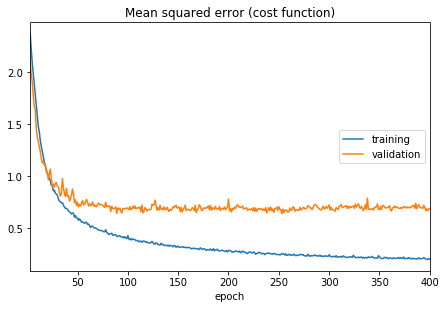
\includegraphics[height=3.3cm]{img/STEP12_7/STEP12_7_pBr2SXR_rm-rs_absarg_training_mse.png} \label{step_12_7_training}}
    \subfigure{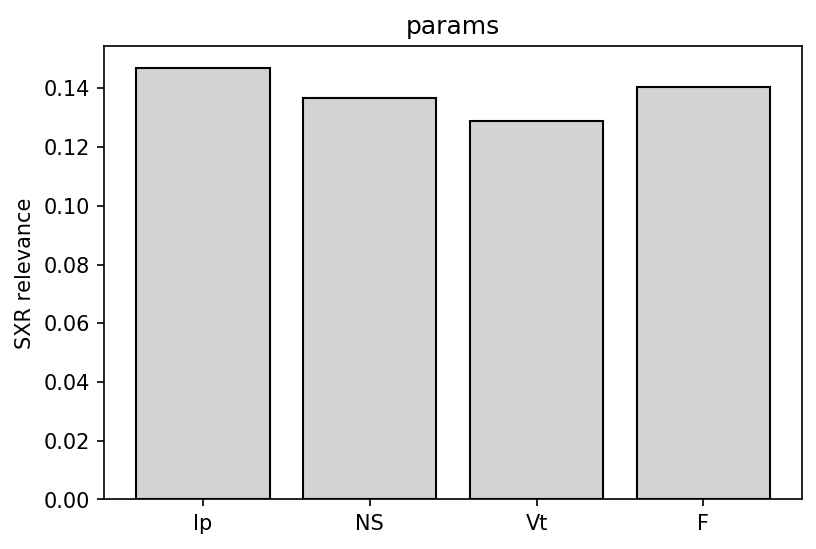
\includegraphics[height=3.3cm]{img/STEP12_7/STEP12_7_params.png} \label{step_12_7_p}}
    \subfigure{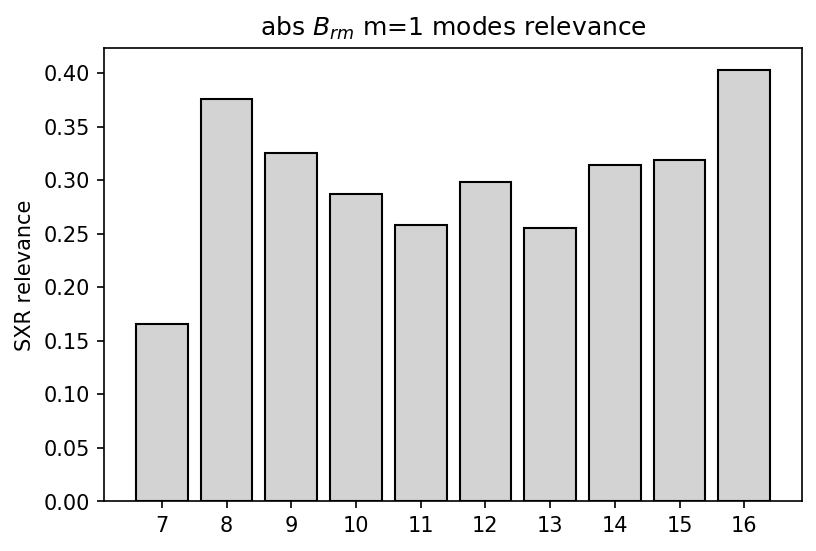
\includegraphics[height=3.3cm]{img/STEP12_7/STEP12_7_abs_Br_rm.png} \label{step_12_7_abs_Brm}}
    \subfigure{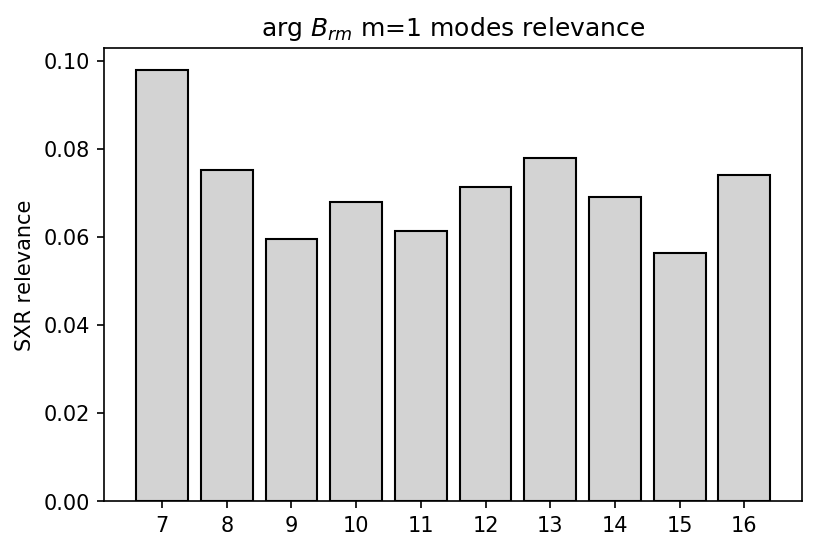
\includegraphics[height=3.3cm]{img/STEP12_7/STEP12_7_arg_Br_rm.png} \label{step_12_7_arg_Brm}}
    \subfigure{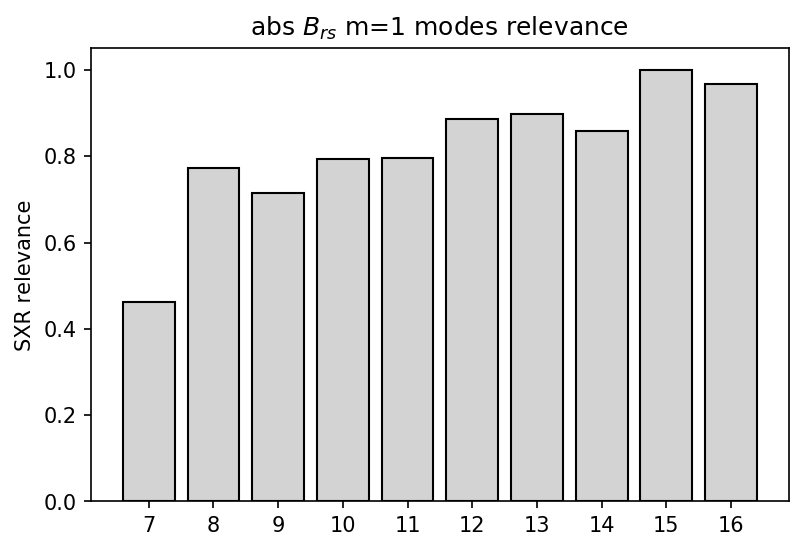
\includegraphics[height=3.3cm]{img/STEP12_7/STEP12_7_abs_Br_rs.png} \label{step_12_7_abs_Brs}}
    \subfigure{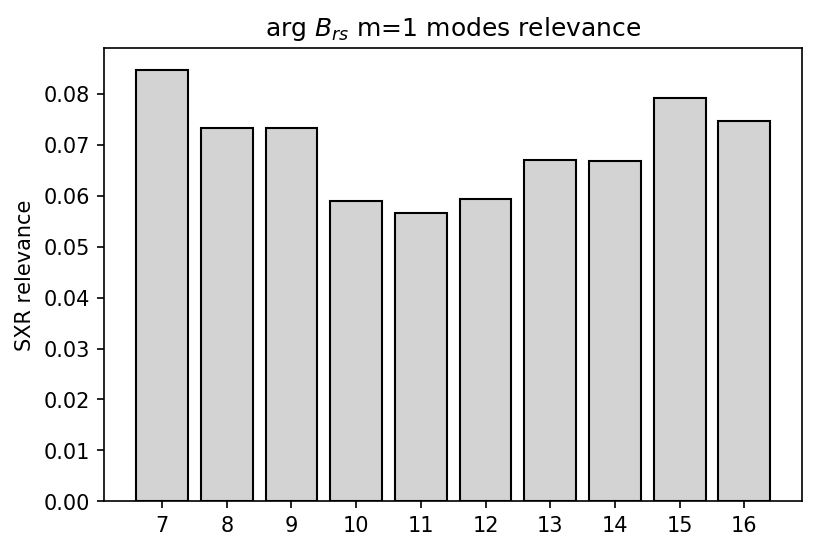
\includegraphics[height=3.3cm]{img/STEP12_7/STEP12_7_arg_Br_rs.png} \label{step_12_7_arg_Brs}}
    \caption{ Training 500 epochs - STEP 12.7 mse, slightly overfitted but validation not diverging }
    \label{fig:step_12_7}
\end{figure}

\begin{figure}
    \centering
    \subfigure{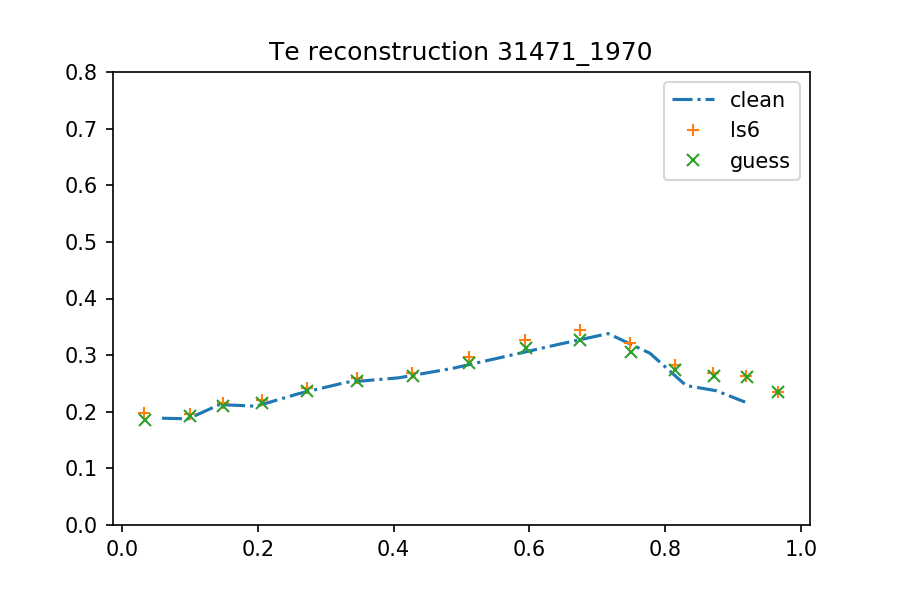
\includegraphics[height=4.8cm]{img/STEP12_7/Te_rec_215.png} }
%   \subfigure{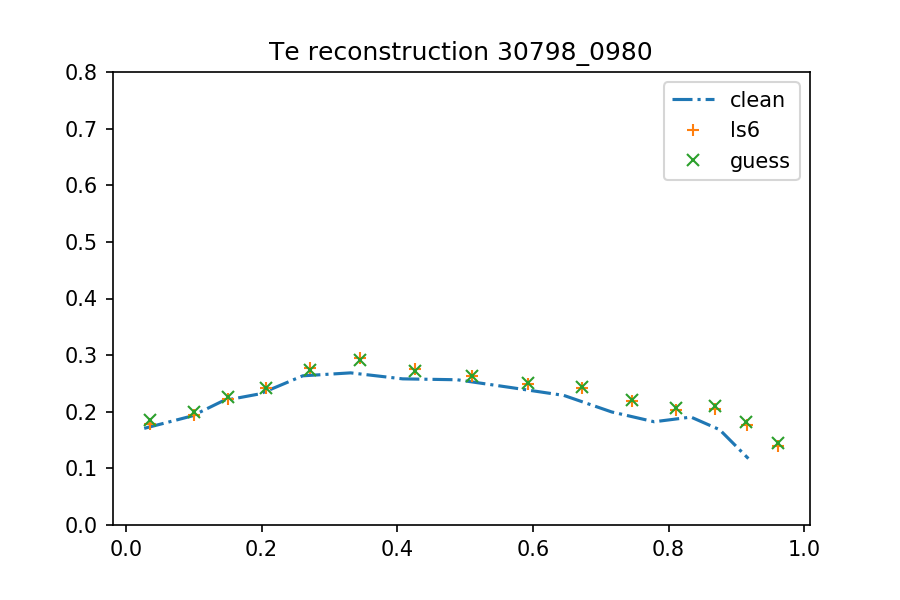
\includegraphics[height=4.8cm]{img/STEP12_7/Te_rec_219.png} }
    \subfigure{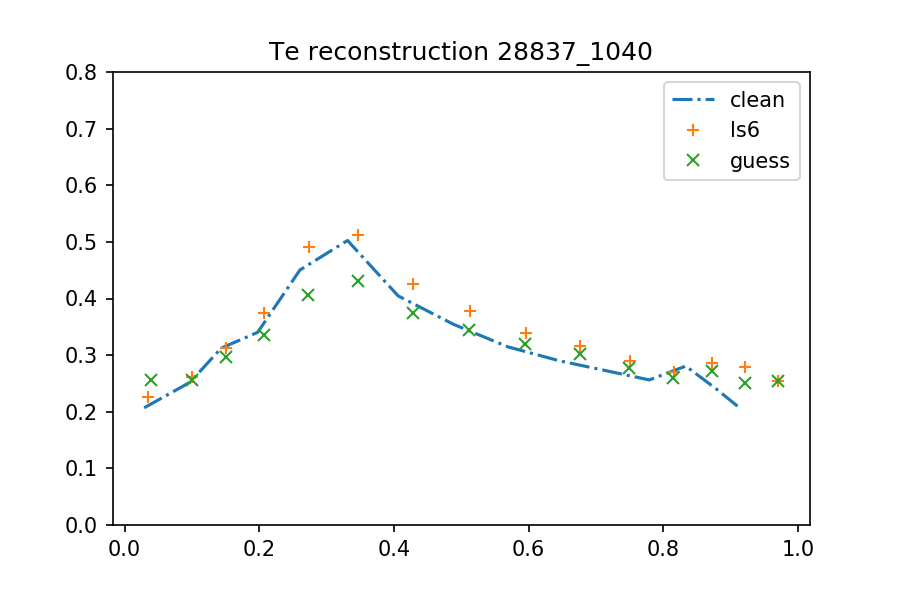
\includegraphics[height=4.8cm]{img/STEP12_7/Te_rec_229.png} }
    \subfigure{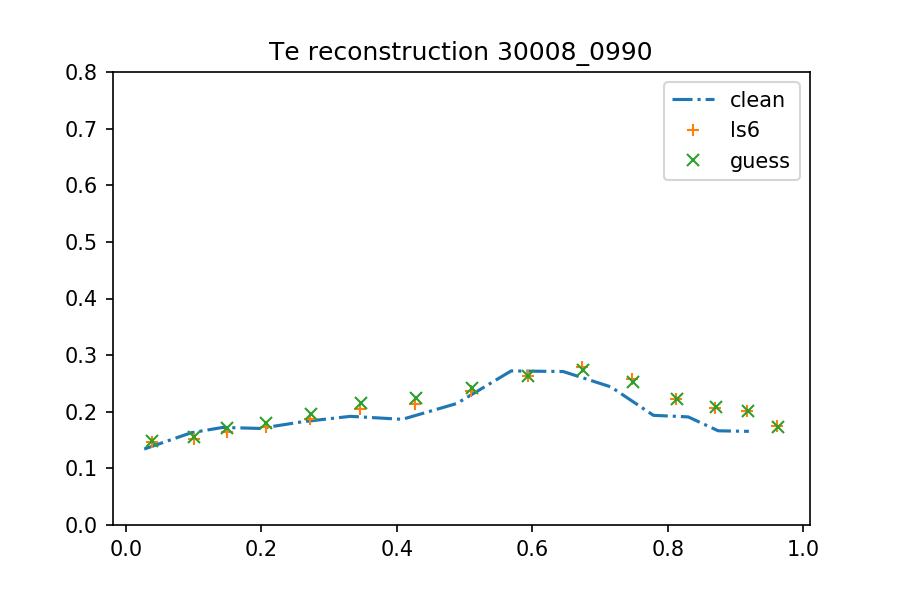
\includegraphics[height=4.8cm]{img/STEP12_7/Te_rec_232.png} }
%   \subfigure{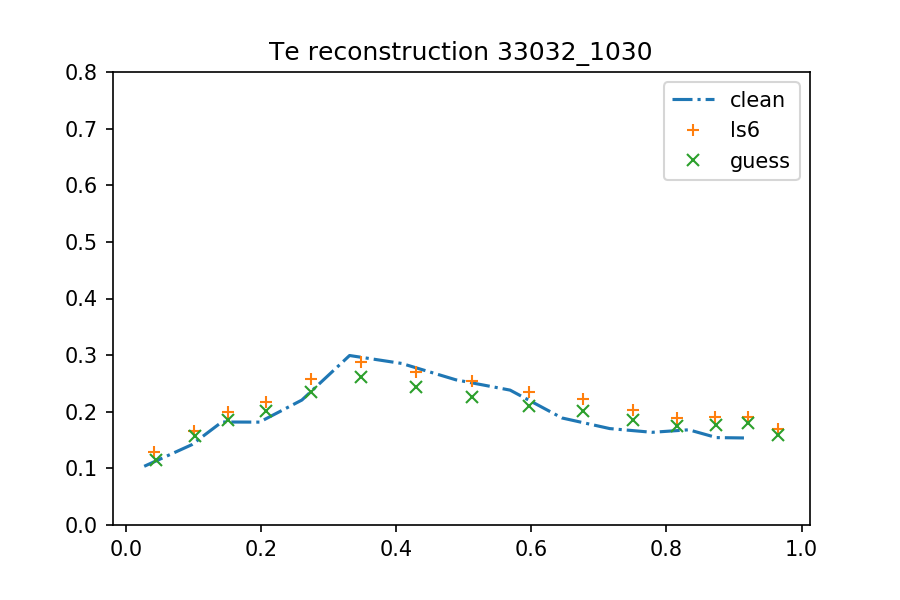
\includegraphics[height=4.8cm]{img/STEP12_7/Te_rec_243.png} }
    \subfigure{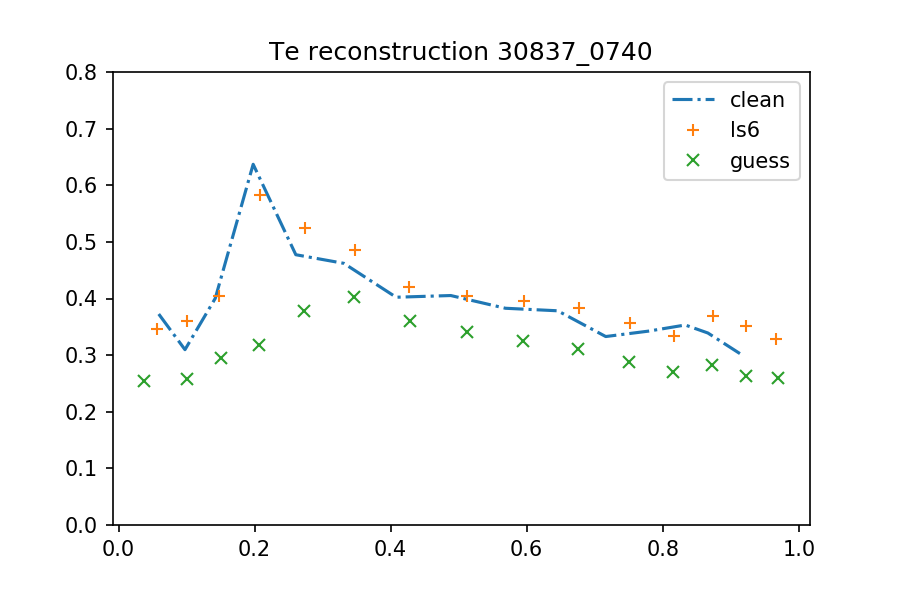
\includegraphics[height=4.8cm]{img/STEP12_7/Te_rec_213.png} }
    \caption{ Training 500 epochs - STEP 12.7 mse, slightly overfitted but validation not diverging }
    \label{fig:step_12_7_rec}
\end{figure}

